\documentclass[../include.tex]{subfiles}
\begin{document}
\chapter{Numerical experiments}
\chaptermark{Numerical experiments}
\section{Viscous Burgers' equation}
In order to test the numerical scheme, we chose 4 representative solutions of the viscous Burgers' equation:
the traveling-wave solution, the rarefaction-wave solution, the triangular-wave solution and a trigonometric solution. In an earlier work \cite{iioe0} the authors have used the traveling-wave solution to test the numerical scheme (\ref{iioe}).\\
\subsection{Traveling wave}
The traveling-wave solution can be obtained by looking for special solutions of the Burgers' equation (\ref{burg}) that are only shifted in time. This way we can obtain
\begin{equation}
	u(x,t) = u_r + \frac{1}{2}(u_l-u_r)\left(1-\tanh \left(\frac{(u_l-u_r)(x-st)}{4 \sigma}\right) \right),
	\label{travel}
\end{equation}
where $ s = (u_l + u_r)/2 $ is the propagation speed. Here we chose $ u_l = 1,\,u_r = 0 $. We will use it as our first example to test the numerical scheme (\ref{iioe}) on space interval $ (-0.5, 0.5) $ and time interval $ (0, 0.48) $.
First we solve the problem with $ \sigma = 0.01 $.
In this test example we chose a time step $ \tau = 4h $. It means that for $ h = 0.01 (n = 100) $ we use a time step $ \tau = 0.04 $. Then one can refine the time step and grid size in order to check that the scheme is second order accurate, cf. Table \ref{tab:travel}. The visual comparisons of the numerical and exact solutions for $ n = 100 $ are presented in Figure \ref{fig:travel}.

It is interesting to consider what happens if we don't perform any nonlinear iteration. Which means that we calculate the inflow coefficients using the values of the solution from the previous time step. This way we get EOC = 1, as it is documented in Table \ref{tab:travel_1iter}. In Figure \ref{fig:travel_iter} we can observe that the propagation speed of the numerical solution differs from the exact one. By refining the grid, the speed gets closer to the exact one.

In the second case we decreased the viscosity to $ \sigma = 0.001 $. In Table \ref{tab:travelsig1/1000} we show errors and EOC for refined and coarsened grids and time step. One can again see that EOC = 2 also in this example when refining the grid. The lower convergence rate in the beginning is caused by oscillations when the grid size is not sufficiently fine, but as we can see from Figure \ref{fig:travel_sig1/1000_n500} these oscillations are ”stable”, they do not increase in time and
by refining the spatial resolution they are removed completely as documented in Figure \ref{fig:travel_sig1/1000_n1000}.

\begin{table}[ht]
	\caption{Report on the $L_2$ errors of $\mathrm{IIOE}$ method for the traveling-wave solution {\rm (\ref{travel})} of the viscous Burgers' equation {\rm (\ref{burg})} with $\sigma = 0.01$. }
	\begin{center} \footnotesize
		\begin{tabular}{|c|c|c|c|c|c|}
			\hline  
			$ n $ & $ h $ & $\tau$ & NTS & $L_2(I,L_2)$ & EOC\\
			\hline
			\lower.3ex\hbox{100} & \lower.3ex\hbox{0.01} & \lower.3ex\hbox{0.04} & \lower.3ex\hbox{12} & \lower.3ex\hbox{5.0 $10^{-3}$} &\\
			\hline
			\lower.3ex\hbox{200} & \lower.3ex\hbox{0.005} & \lower.3ex\hbox{0.02} & \lower.3ex\hbox{24} & \lower.3ex\hbox{1.22 $10^{-3}$} & \lower.3ex\hbox{2.03}\\
			\hline
			\lower.3ex\hbox{400} & \lower.3ex\hbox{0.0025} & \lower.3ex\hbox{0.01} & \lower.3ex\hbox{48} & \lower.3ex\hbox{3.03 $10^{-4}$} & \lower.3ex\hbox{2.01}\\
			\hline
			\lower.3ex\hbox{800} & \lower.3ex\hbox{0.00125} & \lower.3ex\hbox{0.005} & \lower.3ex\hbox{96} & \lower.3ex\hbox{7.74 $10^{-5}$} & \lower.3ex\hbox{1.97}\\
			\hline
			\lower.3ex\hbox{1600} & \lower.3ex\hbox{0.000625} & \lower.3ex\hbox{0.025} & \lower.3ex\hbox{192} & \lower.3ex\hbox{1.90 $10^{-5}$} & \lower.3ex\hbox{2.02}\\
			\hline
		\end{tabular}
	\end{center}
	\label{tab:travel}
\end{table}

\begin{figure}[h!]
	\centering
	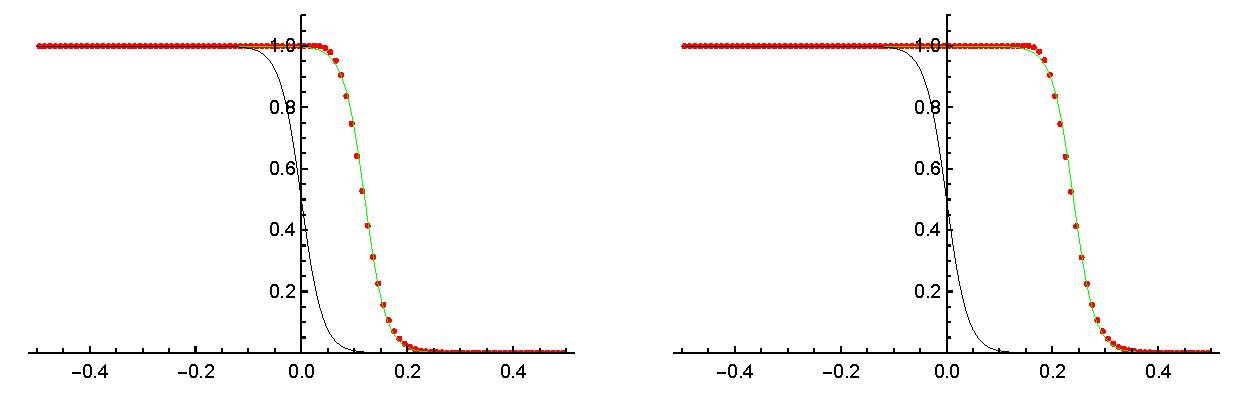
\includegraphics[width=\textwidth]{figures/travel100.pdf}
	\caption{Comparing the $ \mathrm{IIOE} $ scheme with the exact traveling-wave solution {\rm (\ref{travel})} in time $ t=0.24 $ (left) and $ t = 0.48 $ (right), with $ \sigma=0.01 $, $ n=100 $, $ \tau=4h $}
	\label{fig:travel}
\end{figure}

\begin{table}[h!]
	\caption{Report on the $L_2$ errors of $\mathrm{IIOE}$ method for the traveling-wave solution {\rm (\ref{travel})} of the viscous Burgers' equation {\rm (\ref{burg})} with $\sigma = 0.01$, number of nonlinear iterations = 1. }
	\begin{center} \footnotesize
		\begin{tabular}{|c|c|c|c|c|c|}
			\hline  
			$ n $ & $ h $ & $\tau$ & NTS & $L_2(I,L_2)$ & EOC\\
			\hline
			\lower.3ex\hbox{100} & \lower.3ex\hbox{0.01} & \lower.3ex\hbox{0.04} & \lower.3ex\hbox{12} & \lower.3ex\hbox{4.41 $10^{-2}$} &\\
			\hline
			\lower.3ex\hbox{200} & \lower.3ex\hbox{0.005} & \lower.3ex\hbox{0.02} & \lower.3ex\hbox{24} & \lower.3ex\hbox{2.32 $10^{-2}$} & \lower.3ex\hbox{0.93}\\
			\hline
			\lower.3ex\hbox{400} & \lower.3ex\hbox{0.0025} & \lower.3ex\hbox{0.01} & \lower.3ex\hbox{48} & \lower.3ex\hbox{1.18 $10^{-2}$} & \lower.3ex\hbox{0.97}\\
			\hline
			\lower.3ex\hbox{800} & \lower.3ex\hbox{0.00125} & \lower.3ex\hbox{0.005} & \lower.3ex\hbox{96} & \lower.3ex\hbox{5.96 $10^{-3}$} & \lower.3ex\hbox{0.99}\\
			\hline
		\end{tabular}
	\end{center}
	\label{tab:travel_1iter}
\end{table}

\begin{figure}[h!]
	\centering
	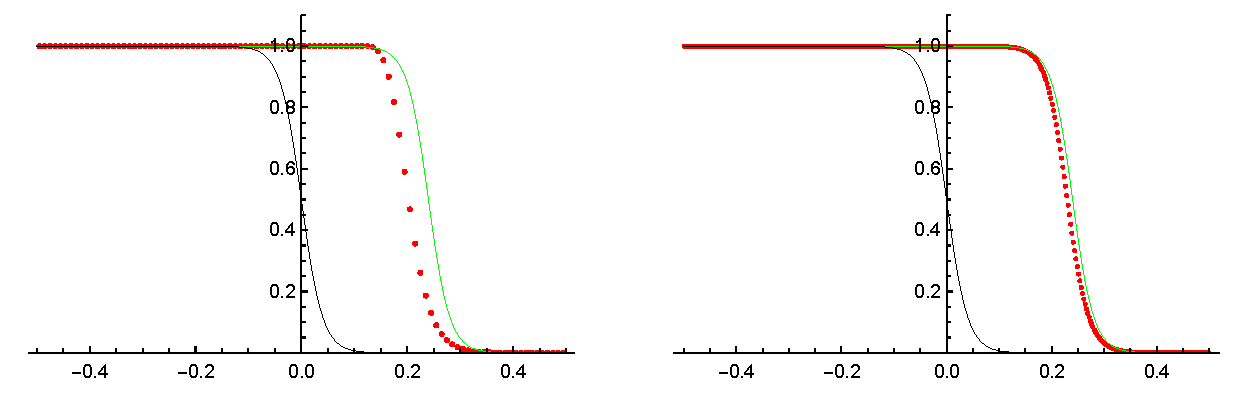
\includegraphics[width=\textwidth]{figures/traveliter}
	\caption{Comparing the $ \mathrm{IIOE} $ scheme with the exact traveling-wave solution {\rm (\ref{travel})} in time $ t=0.48 $, with $ \sigma=0.01 $, $ n=100 $(left), $ n=400 $(right), $ \tau=4h $, $ \textrm{number of nonlinear iterations} = 1 $. We can see that after refining the grid, the propagation speed of the numerical solution is getting closer to the exact speed.}
	\label{fig:travel_iter}
\end{figure}

\begin{table}[h!]
	\caption{Report on the $L_2$ errors of $\mathrm{IIOE}$ method for the traveling-wave solution {\rm (\ref{travel})}  of the viscous Burgers' equation {\rm (\ref{burg})}  with $\sigma = 0.001$. }
	\begin{center} \footnotesize
		\begin{tabular}{|c|c|c|c|c|c|}
			\hline  
			$ n $ & $ h $ & $\tau$ & NTS & $L_2(I,L_2)$ & EOC\\
			\hline
			\lower.3ex\hbox{250} & \lower.3ex\hbox{0.004} & \lower.3ex\hbox{0.016} & \lower.3ex\hbox{30} & \lower.3ex\hbox{2.01 $10^{-2}$} &\\
			\hline
			\lower.3ex\hbox{500} & \lower.3ex\hbox{0.002} & \lower.3ex\hbox{0.08} & \lower.3ex\hbox{60} & \lower.3ex\hbox{6.84 $10^{-3}$} & \lower.3ex\hbox{1.55}\\
			\hline
			\lower.3ex\hbox{1000} & \lower.3ex\hbox{0.001} & \lower.3ex\hbox{0.04} & \lower.3ex\hbox{120} & \lower.3ex\hbox{1.79 $10^{-3}$} & \lower.3ex\hbox{1.94}\\
			\hline
			\lower.3ex\hbox{2000} & \lower.3ex\hbox{0.0005} & \lower.3ex\hbox{0.02} & \lower.3ex\hbox{240} & \lower.3ex\hbox{4.55 $10^{-4}$} & \lower.3ex\hbox{1.97}\\
			\hline
		\end{tabular}
	\end{center}
	\label{tab:travelsig1/1000}
\end{table}

\begin{figure}[h!]
	\centering
	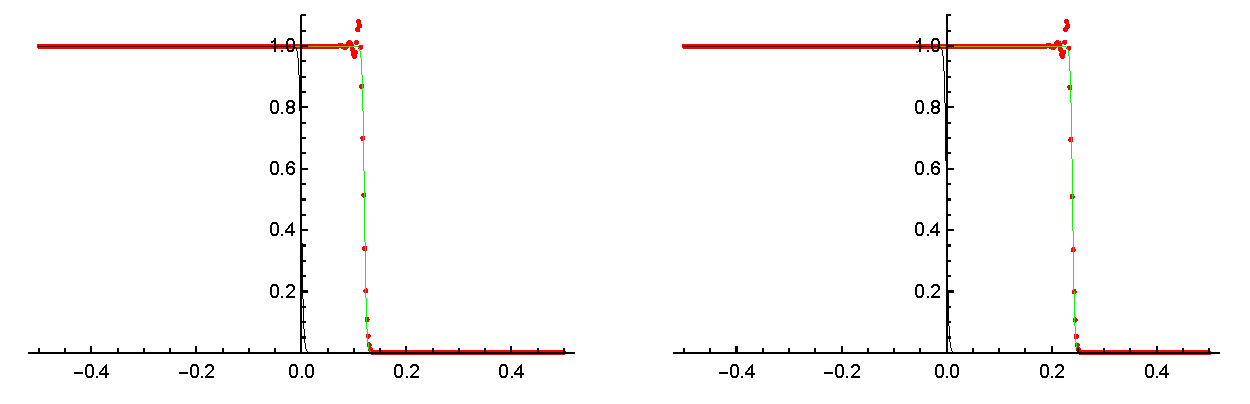
\includegraphics[width=\textwidth]{figures/travelsig0015002448}
	\caption{Comparing the $ \mathrm{IIOE} $ scheme with the exact traveling-wave solution {\rm (\ref{travel})} in time $ t=0.24 $ (left) and $ t = 0.48 $ (right), with $ \sigma=0.001 $, $ n=500 $, $ \tau=4h $. We can observe small nonincreasingly propagating oscillations.}
	\label{fig:travel_sig1/1000_n500}
\end{figure}

\begin{figure}[h!]
	\centering
	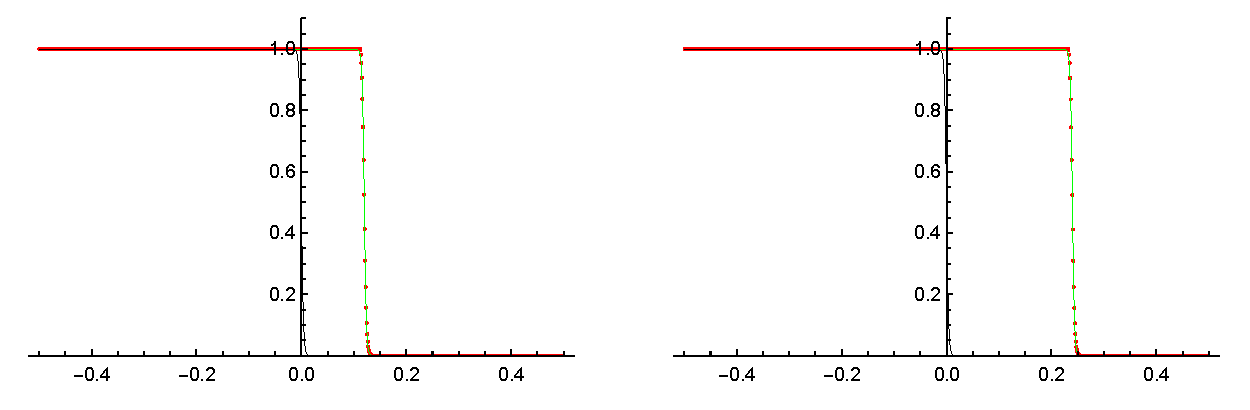
\includegraphics[width=\textwidth]{figures/travelsig0011000024048}
	\caption{Comparing the $ \mathrm{IIOE} $ scheme with the exact traveling-wave solution {\rm (\ref{travel})} in time $ t=0.24 $ (left) and $ t = 0.48 $ (right), with $ \sigma=0.001 $, $ n=1000 $, $ \tau=4h $. On the refined grid the oscillations are gone.}
	\label{fig:travel_sig1/1000_n1000}
\end{figure}
%====================================================================================================================================================
\newpage
\subsection{Rarefaction wave}
The next example is the rarefaction-wave solution \eqref{rare}. We chose $ u_l = 0,\,u_r = 1 $ and $ \sigma = 0.01 $. First, equation (\ref{burg}) is solved by the scheme (\ref{iioe}) on space interval $ (-0.5, 0.5) $ and time interval $ [0.01, 0.41) $. Since the exact solution (\ref{rare}) is defined for $ t>0 $, we decided to initialize the calculation at time 0.01. The time step $ \tau $ was chosen to be equal to $ 4h $ again. The numerical solution is visually compared to the exact solution in Figure \ref{fig:rare}. The errors are presented in Table \ref{tab:rare}.

\begin{table}[h!]
	\caption{Report on the $L_2$ errors of $\mathrm{IIOE}$ method for the rarefaction-wave solution {\rm (\ref{rare})} of the viscous Burgers' equation {\rm (\ref{burg})} with $\sigma = 0.01$. }
	\begin{center} \footnotesize
		\begin{tabular}{|c|c|c|c|c|c|}
			\hline  
			$ n $ & $ h $ & $\tau$ & NTS & $L_2(I,L_2)$ & EOC\\
			\hline
			\lower.3ex\hbox{100} & \lower.3ex\hbox{0.01} & \lower.3ex\hbox{0.04} & \lower.3ex\hbox{10} & \lower.3ex\hbox{5.48 $10^{-3}$} &\\
			\hline
			\lower.3ex\hbox{200} & \lower.3ex\hbox{0.005} & \lower.3ex\hbox{0.02} & \lower.3ex\hbox{20} & \lower.3ex\hbox{1.56 $10^{-3}$} & \lower.3ex\hbox{1.82}\\
			\hline
			\lower.3ex\hbox{400} & \lower.3ex\hbox{0.0025} & \lower.3ex\hbox{0.01} & \lower.3ex\hbox{40} & \lower.3ex\hbox{4.01 $10^{-4}$} & \lower.3ex\hbox{1.96}\\
			\hline
			\lower.3ex\hbox{800} & \lower.3ex\hbox{0.00125} & \lower.3ex\hbox{0.005} & \lower.3ex\hbox{80} & \lower.3ex\hbox{1.00 $10^{-4}$} & \lower.3ex\hbox{2.00}\\
			\hline
		\end{tabular}
	\end{center}
	\label{tab:rare}
\end{table}

\begin{figure}[h!]
	\centering
	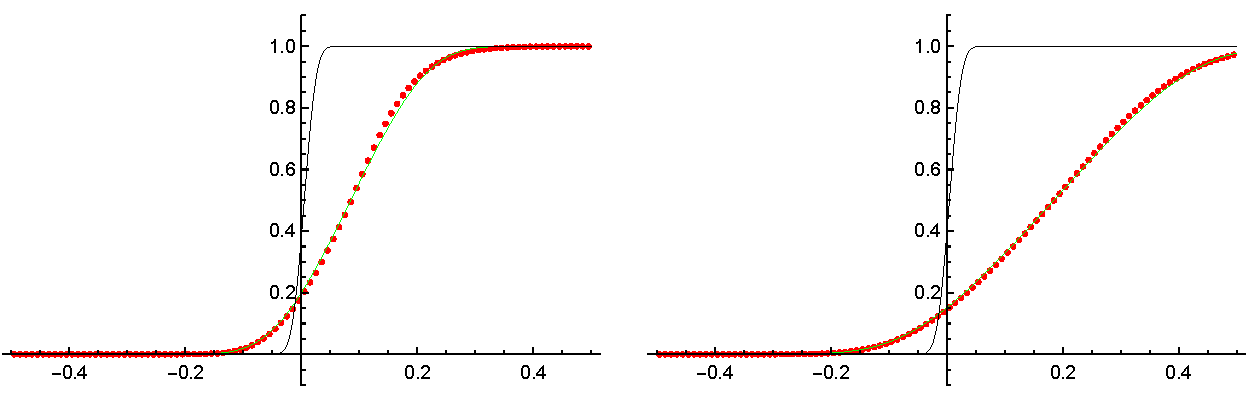
\includegraphics[width=\textwidth]{figures/rare100}
	\caption{Comparing the $\mathrm{IIOE}$ scheme with the exact rarefaction-wave solution {\rm (\ref{rare})} in time $ t=0.17 $ (left) and $ t = 0.41 $ (right), with $ \sigma=0.01 $, $ n=100 $, $ \tau=4h $}
	\label{fig:rare}
\end{figure}
%====================================================================================================================================================
\newpage
\subsection{Triangular wave}
Our third example is the triangular-wave solution \eqref{triang}. In this case the problem (\ref{burg}) is solved by the scheme (\ref{iioe}) on space interval $ (-0.5, 1.5) $ and time interval $ (0.01, 0.51) $ with $ \sigma = 0.02 $. Again, the exact solution (\ref{triang}) is defined for $ t > 0 $ so the numerical calculation was initialized at time 0.01. In Table \ref{ttri} we show the errors for refined grids and time step. When the grid size is not sufficiently fine, we can observe oscillations at the peak of the wave \ref{fig:triang-osc}. These oscillations do not grow unboundedly and can be removed by refining the grid as it is shown in Figure \ref{ftri1}.

\begin{table}[ht]
	\caption{Report on the $L_2$ errors of $\mathrm{IIOE}$ method for the triangular-wave solution {\rm (\ref{triang})} of the viscous Burgers' equation {\rm (\ref{burg})} with $\sigma = 0.02$. }
	\begin{center} \footnotesize
		\begin{tabular}{|c|c|c|c|c|c|}
			\hline  
			$n$ & $h$ & $\tau$ & \lower.3ex\hbox{NTS} & \lower.3ex\hbox{$L_2(I,L_2)$} & \lower.3ex\hbox{EOC}\\
			\hline
			\lower.3ex\hbox{100} & \lower.3ex\hbox{0.02} & \lower.3ex\hbox{0.08} & \lower.3ex\hbox{5} & \lower.3ex\hbox{3.07 $10^{-1}$} &\\
			\hline
			\lower.3ex\hbox{200} & \lower.3ex\hbox{0.01} & \lower.3ex\hbox{0.04} & \lower.3ex\hbox{10} & \lower.3ex\hbox{1.30 $10^{-1}$} &\lower.3ex\hbox{1.24}\\
			\hline
			\lower.3ex\hbox{400} & \lower.3ex\hbox{0.005} & \lower.3ex\hbox{0.02} & \lower.3ex\hbox{20} & \lower.3ex\hbox{3.72 $10^{-2}$} &\lower.3ex\hbox{1.81}\\
			\hline
			\lower.3ex\hbox{800} & \lower.3ex\hbox{0.0025} & \lower.3ex\hbox{0.01} & \lower.3ex\hbox{40} & \lower.3ex\hbox{9.02 $10^{-3}$} &\lower.3ex\hbox{2.04}\\
			\hline
		\end{tabular}
	\end{center}
	\label{ttri}
\end{table}

\begin{figure}[h!]
	\centering
	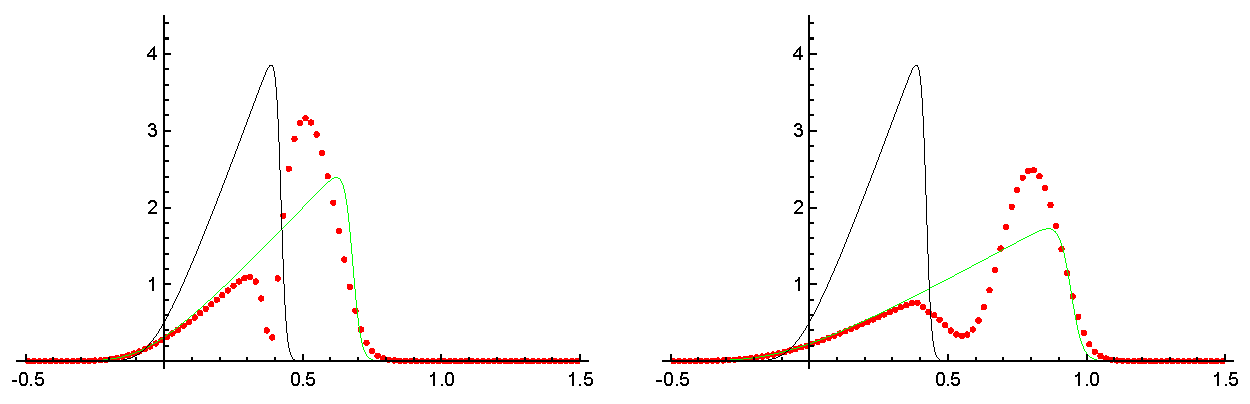
\includegraphics[width=\textwidth]{figures/tri100.pdf}
	\caption{Comparing the $\mathrm{IIOE}$ scheme with the exact traingular wave solution {\rm (\ref{triang})} in time $ t = 0.26 $ (left), $ t = 0.50 $ (right) for $ n=100 $, whith $ \sigma=0.02 $,  $ \tau = 4h $.}
	\label{fig:triang-osc}
\end{figure}

\begin{figure}[h]
	\centering
	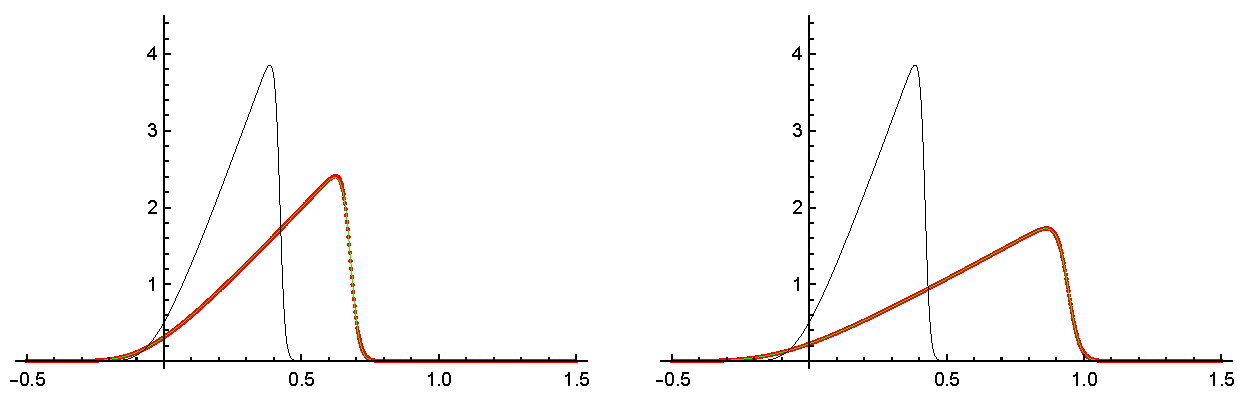
\includegraphics[width=\textwidth]{figures/tri800.pdf}
	\caption{Comparing the $\mathrm{IIOE}$ scheme with the exact traingular wave solution {\rm (\ref{triang})} in time $ t = 0.26 $ (left), $ t = 0.50 $ (right) for $ n=800 $ whith $ \sigma=0.02 $,  $ \tau = 4h $.}
	\label{fig:triang}
\end{figure}

%====================================================================================================================================================

\subsection{Trigonometric solution}
Our last example is the trigonometric solution \eqref{trig} with $ a = 1.0025,\,b=1,\,\lambda = \pi^2 $ and $ \sigma = 0.01 $.
%\begin{equation}
%	u(x,t)=\frac{2\sigma b \pi \sin{\pi x}}{ae^{\sigma \pi^{2}t}+b\cos \pi x },
%\end{equation}
The errors are reported in Table \ref{ttrig}. A visual comparison of the numerical results with the exact solution is presented in Figure \ref{ftrig}.

\begin{table}[h!]
	\caption{Report on the $L_2$ errors of $\mathrm{IIOE}$ method for the trigonometric solution {\rm (\ref{trig})} of the viscous Burgers' equation {\rm (\ref{burg})} with $\sigma = 0.01$. }
	\begin{center} \footnotesize
		\begin{tabular}{|c|c|c|c|c|c|}
			\hline
			$n$ & $h$& $\tau$ & NTS & $L_2(I,L_2)$ & EOC\\
			\hline
			\lower.3ex\hbox{100} & \lower.3ex\hbox{0.02} & \lower.3ex\hbox{0.08} & \lower.3ex\hbox{15} & \lower.3ex\hbox{1.66 $10^{-2}$} &\\
			\hline
			\lower.3ex\hbox{200} & \lower.3ex\hbox{0.01} & \lower.3ex\hbox{0.04} & \lower.3ex\hbox{30} & \lower.3ex\hbox{3.18 $10^{-3}$} &\lower.3ex\hbox{2.38}\\
			\hline
			\lower.3ex\hbox{400} & \lower.3ex\hbox{0.005} & \lower.3ex\hbox{0.02} & \lower.3ex\hbox{60} & \lower.3ex\hbox{5.30 $10^{-4}$} &\lower.3ex\hbox{2.58}\\
			\hline
			\lower.3ex\hbox{800} & \lower.3ex\hbox{0.0025} & \lower.3ex\hbox{0.01} & \lower.3ex\hbox{120} & \lower.3ex\hbox{1.00 $10^{-4}$} &\lower.3ex\hbox{2.41}\\
			\hline
		\end{tabular}
	\end{center}
	\label{ttrig}
\end{table}

\begin{figure}[h!] 
	\centering
	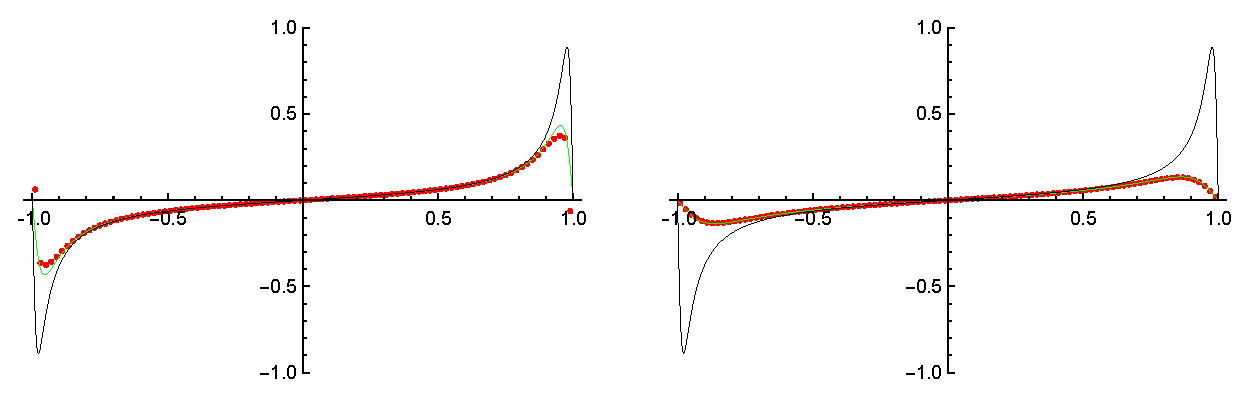
\includegraphics[width=\textwidth]{figures/trig100}
	\caption{Comparing the $\mathrm{IIOE}$ scheme with the exact trigonometric solution {\rm (\ref{trig})} in time $ t = 0.08 $ (left) and $ t = 0.96 $ (right) for $ n=100 $, with $ \sigma=0.01 $, $ b=1 $, $ a=1.0025 $, $ \tau = 4h $.}
	\label{ftrig} 
\end{figure} 

%====================================================================================================================================================
\newpage
\section{Traffic flow}
In this section we solve the traffic flow equation \eqref{traffic} with $ v_{max} = 1 $.
As discussed earlier, by making certain assumptions about the flux function, we can transform the solutions of viscous Burgers' equation \eqref{burg} to obtain a solution for the density of the cars in the traffic flow problem (\ref{traffic}). Below we give an interpretation of the traveling-wave and the rarefaction-wave solution in a traffic flow context.

\subsection{Traveling wave}
A traveling wave can form in a traffic, when incoming cars are approaching a congestion or a line of cars staying behind a red light waiting for turning to green. In the congestion, the density $ \rho_r = 1 $, which means bumper to bumper traffic. The density of the incoming traffic was chosen to be $ \rho_r = 0.1 $, which means that there is one car/10 car lengths.

The exact solution for the density was obtained as follows: considering the densities $ \rho_l = 0,\,\rho_l = 1 $ and using the relationship \eqref{u-ro} we can calculate $ u_l = 0.8$ and $ u_r = -1 $ for the traveling wave solution \eqref{travel} of the Burgers' equation. Then using the relationship (\ref{ro-u}) we obtain the solution for the density. This solution for the traffic density $ \rho $ was compared to the numerical solution using the IIOE scheme (\ref{iioe}). The errors are documented in Table \ref{tab:density_travel_sig1/1000}. The solution for $ D = 0.01 $ is presented in Figure \ref{fig:traffic_travel}.
\begin{table}[h!]
	\caption{Report on the $L_2$ errors of $\mathrm{IIOE}$ method for the traffic flow problem {\rm (\ref{traffic})} with $ D = 0.01$. }
	\begin{center} \footnotesize
		\begin{tabular}{|c|c|c|c|c|c|}
			\hline  
			$ n $ & $ h $ & $\tau$ & NTS & $L_2(I,L_2)$ & EOC\\
			\hline
			\lower.3ex\hbox{100} & \lower.3ex\hbox{0.01} & \lower.3ex\hbox{0.04} & \lower.3ex\hbox{12} & \lower.3ex\hbox{9.82 $10^{-4}$} &\\
			\hline
			\lower.3ex\hbox{200} & \lower.3ex\hbox{0.005} & \lower.3ex\hbox{0.02} & \lower.3ex\hbox{24} & \lower.3ex\hbox{2.36 $10^{-4}$} & \lower.3ex\hbox{2.05}\\
			\hline
			\lower.3ex\hbox{400} & \lower.3ex\hbox{0.0025} & \lower.3ex\hbox{0.01} & \lower.3ex\hbox{48} & \lower.3ex\hbox{5.94 $10^{-5}$} & \lower.3ex\hbox{1.99}\\
			\hline
			\lower.3ex\hbox{800} & \lower.3ex\hbox{0.00125} & \lower.3ex\hbox{0.005} & \lower.3ex\hbox{96} & \lower.3ex\hbox{1.53 $10^{-5}$} & \lower.3ex\hbox{1.96}\\
			\hline
		\end{tabular}
	\end{center}
	\label{tab:density_travel_sig1/1000}
\end{table}
\begin{figure}[h!]
	\centering
	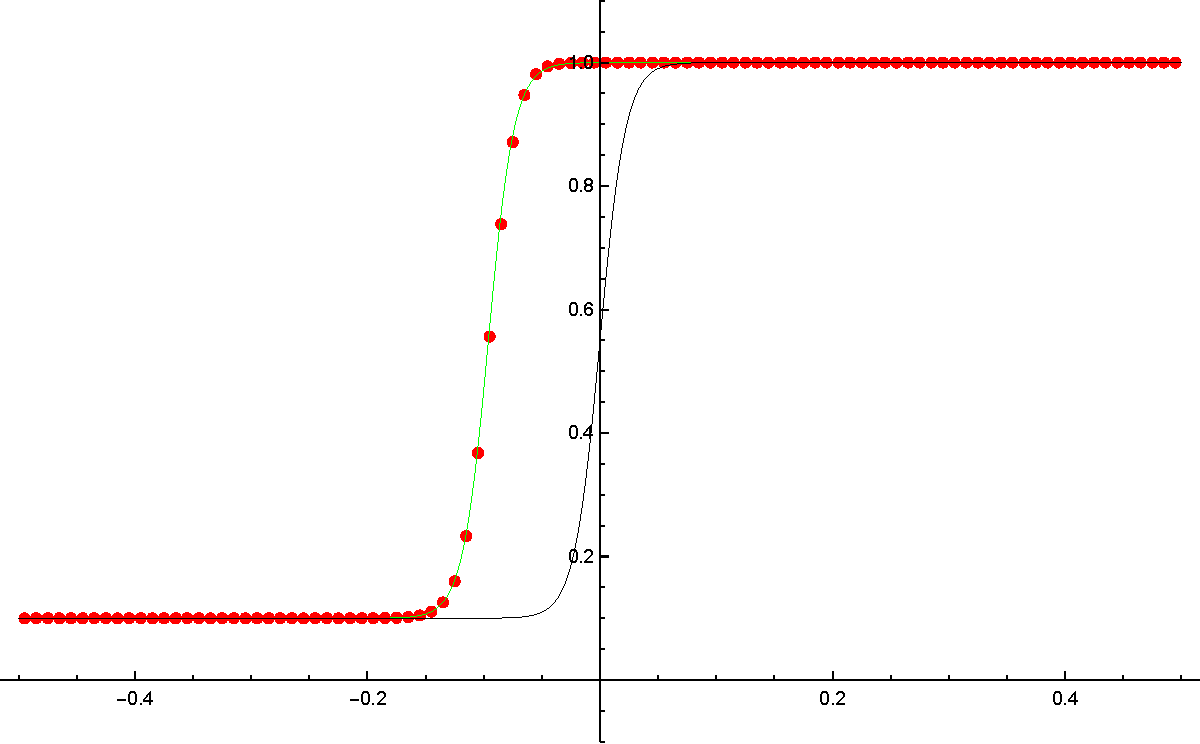
\includegraphics[width=.5\textwidth]{figures/trafficTravel100t.96}
	\caption{Cars from left with traffic density $ \rho_l = 0.1 $ are approaching the congested region with $ \rho_r = 1 $. This would happen, for example, when cars are staying behind a red light. 
		The blue line is the initial condition for the numerical computation, the red dots are the values computed by the IIOE scheme. The green line is the exact solution obtained by transforming the traveling-wave solution {\rm (\ref{travel})} of the Burgers' equation {\rm (\ref{burg})}(left) using {\rm (\ref{ro-u})}. The results of the numerical solution are shown at time $ t = 0.96 $, for $ n = 100 $, $ \tau = 4h $, $ D = 0.01 $.
	}
	\label{fig:traffic_travel}
\end{figure}

%====================================================================================================================================================
\newpage
\subsection{Rarefaction wave}
We also interpret the rarefaction wave solution in a traffic flow context. Imagine that the road is divided into two parts by the traffic light positioned at the origin. Cars to the left are staying behind the red light for $ t<0 $, so the density $ \rho_l = 1 $ there. On the right there is an empty road, $ \rho_r = 0 $. At time $ t = 0 $ the light turns green. This corresponds to the initial condition for a traffic light positioned at $ x = 0 $
\begin{equation}
	\rho(0,x) =
	\begin{cases}
		1, &x\leq 0,\nonumber\\
		0, &x>0,\nonumber
	\end{cases}
\end{equation}
Right after the light turned green, the cars start to leave, the traffic rarifies. The exact solution for the density in (\ref{trafficonR}) was obtained the same way as in our previous example. First, considering the values $ \rho_l = 1 $, $ \rho_r = 0 $ we calculate the corresponding values $ u_l = -1 $, $ u_r = 1 $ according to (\ref{u-ro}) for the rarefaction wave solution of the Burgers' equation. Then substituting the exact solution (\ref{rare}) to (\ref{ro-u}) we get the density function. The numerical solution for the density by the IIOE scheme (\ref{iioe}) is presented for $ \sigma = 0.01 $ in Figure \ref{fig:traffic_rare}.

\begin{figure}[h!]
	\centering
	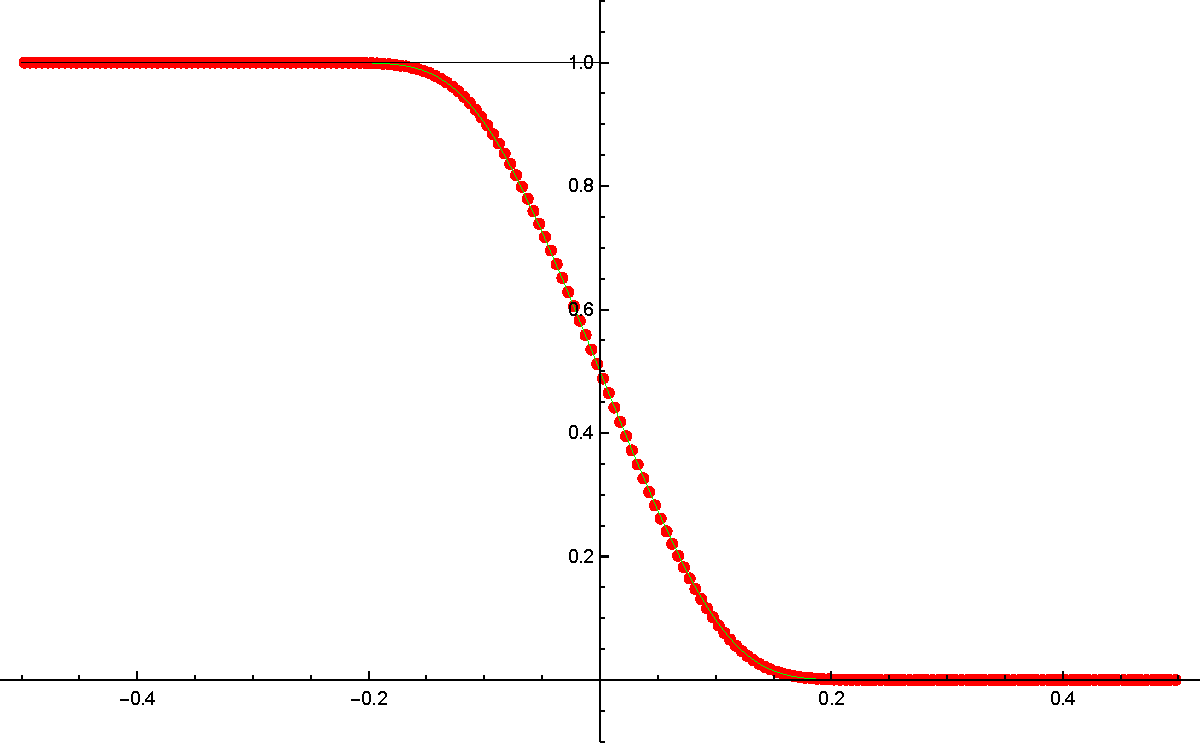
\includegraphics[width=.5\textwidth]{figures/trafficRare1}
	\caption{At $ t<0 $ cars to the left of the origin are staying behind a red light, the density $ \rho_l = 1 $. To the right there is an empty road, $ \rho_r = 0 $. At time $ t = 0 $ the traffic light at the origin turns green and cars start to leave. The black line is the initial condition. At time $ t = 0.08 $ the exact solution(green) is compared to the values obtained by numerical computation(red) for $ n = 100 $, $ \tau = h $, $ D = 0.01 $. The exact solution for the density of cars was obtained by transforming the rarefaction-wave solution {\rm (\ref{rare})} of the Burgers' equation {\rm (\ref{burg})} using {\rm (\ref{ro-u})}.}
	\label{fig:traffic_rare}
\end{figure}
%======================================================================================================================================================================================
\section{Conservation laws}
In the last section we show numerical experiments performed with the basic and the limited IIOE scheme for 1D scalar linear and nonlinear conservation laws.
\subsection{Advection with constant velocity}
The flux limited scheme in the linear case \eqref{advection_limit} is compared with the stabilized schemes $ \mathrm{S^1IIOE} $ (without quadratic reconstruction) and $ \mathrm{S^2IIOE} $ (with quadratic reconstruction) described in \cite{iioe1,iioe2}. For this purpose we use the same examples that can be found in these works: a smooth profile with initial condition $ u_0(x) = \mathrm{max}(0, \cos^5(\pi(x+0.5))) $ and a piecewise constant profile $ u_0(x) = 1 $ for $ x\in[-0.75, -0.25] $, otherwise $ u_0(x) = 0 $. In both cases we solve \eqref{advection_constant} numerically with $ v = 1 $ on space interval $ (-1,1) $ and time interval $ (0,1) $. The exact solution is calculated as $ u(t, x) = u_0(x - t) $.\\
We deal only with the case $ \tau = h $. As noted above, for integer values of the Courant number the errors are the same. The values for $ \mathrm{S^2IIOE} $ (with quadratic reconstruction) are taken from previous works \cite{iioe1,iioe2}.\\
For the smooth profile we can observe that the flux limited scheme performs better than the $ \mathrm{S^1IIOE} $ and it is comparable with the $ \mathrm{S^2IIOE} $ in all cases. The results are documented in \ref{tab:siioe_hump}. In \ref{fig:compare_S1FL_hump} we compare $ \mathrm{S^1IIOE} $ with the flux limited scheme visually.\\
In the case of a discontinous profile the flux limited shceme performs better than both stabilized scheme, c.f.\ \ref{tab:siioe_disc}. A visual comparison with $ \mathrm{S^1 IIOE} $ can be seen in \ref{fig:compare_S1FL_disc}.
\begin{table}[ht]
	\caption{Report on the $L_1$ errors of the $\mathrm{S^1 IIOE}$ (without quadratic reconstruction), $\mathrm{S^2 IIOE}$ (with quadratic reconstruction) and the $\mathrm{FLIIOE}$(flux limited) schemes for a smooth hump, $ \tau = h $.}
	\begin{center} \footnotesize
		\begin{tabular}{|c|c|c|c|c|c|c|}
			\hline
			& $ \mathrm{S^1 IIOE} $ &$ \mathrm{S^1 IIOE} $ & $ \mathrm{S^2 IIOE} $ &$ \mathrm{S^2 IIOE} $ & $ \mathrm{FLIIOE} $ & $ \mathrm{FLIIOE} $ \\
			$ n $ & $\mathrm{L_1(I, L_1)}$ & EOC & $\mathrm{L_1(I, L_1)}$ & EOC & $\mathrm{L_1(I, L_1)}$ & EOC \\
			\hline
			\lower.3ex\hbox{40} &  \lower.3ex\hbox{9.82 $10^{-2}$} & & \lower.3ex\hbox{9.19 $10^{-2}$} & & \lower.3ex\hbox{7.51 $10^{-2}$} &\\
			\hline
			\lower.3ex\hbox{80} &  \lower.3ex\hbox{3.38 $10^{-2}$} &\lower.3ex\hbox{1.54} & \lower.3ex\hbox{2.80 $10^{-2}$} &\lower.3ex\hbox{1.71}&\lower.3ex\hbox{2.66 $10^{-2}$}& \lower.3ex\hbox{1.50} \\
			\hline
			\lower.3ex\hbox{160} &  \lower.3ex\hbox{1.01 $10^{-2}$} &\lower.3ex\hbox{1.74}& \lower.3ex\hbox{7.69 $10^{-3}$} &\lower.3ex\hbox{1.86} &\lower.3ex\hbox{7.55 $10^{-3}$}& \lower.3ex\hbox{1.82} \\
			\hline
			\lower.3ex\hbox{320} &  \lower.3ex\hbox{2.73 $10^{-3}$} &\lower.3ex\hbox{1.89}& \lower.3ex\hbox{1.97 $10^{-3}$} &\lower.3ex\hbox{1.96} &\lower.3ex\hbox{1.96 $10^{-3}$}& \lower.3ex\hbox{1.95}\\
			\hline
			\lower.3ex\hbox{640} &  \lower.3ex\hbox{7.11 $10^{-4}$} &\lower.3ex\hbox{1.94}& \lower.3ex\hbox{4.97 $10^{-4}$} &\lower.3ex\hbox{1.99} &\lower.3ex\hbox{5.22 $10^{-4}$}& \lower.3ex\hbox{1.91} \\
			\hline
			\lower.3ex\hbox{1280} &  \lower.3ex\hbox{1.83 $10^{-4}$} &\lower.3ex\hbox{1.96}& \lower.3ex\hbox{1.24 $10^{-4}$} &\lower.3ex\hbox{2.00} &\lower.3ex\hbox{1.41 $10^{-4}$}& \lower.3ex\hbox{1.89} \\
			\hline
		\end{tabular}
	\end{center}
	\label{tab:siioe_hump}
\end{table}

\begin{figure}[H]
	\centering
	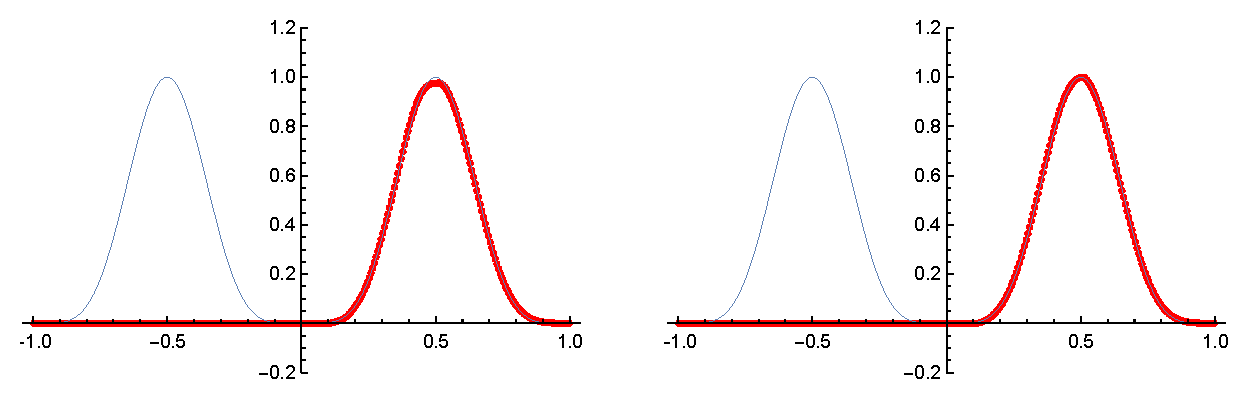
\includegraphics[width=\textwidth]{figures/compareHump.pdf}
	\caption{Comparing the $\mathrm{S^1 IIOE}$ (without quadratic reconstruction) and the $\mathrm{FLIIOE}$ schemes with the exact solution  in time $ t=1 $, $ n=320 $, $ \tau=h $.}
	\label{fig:compare_S1FL_hump}
\end{figure}

\begin{table}[ht]
	\caption{Report on the $L_1$ errors of the $\mathrm{S^1 IIOE}$ (without quadratic reconstruction), $\mathrm{S^2 IIOE}$ (with quadratic reconstruction) and the $\mathrm{FLIIOE}$(flux limited) schemes for a discontinous piecewise profile, $ \tau = h $.}
	\begin{center} \footnotesize
		\begin{tabular}{|c|c|c|c|c|c|c|}
			\hline
			& $ \mathrm{S^1 IIOE} $ &$ \mathrm{S^1 IIOE} $ & $ \mathrm{S^2 IIOE} $ &$ \mathrm{S^2 IIOE} $ & $ \mathrm{FLIIOE} $ & $ \mathrm{FLIIOE} $ \\
			$ n $ & $\mathrm{L_1 error}$ & EOC & $\mathrm{L_1 error}$ & EOC & $\mathrm{L_1 error}$ & EOC \\
			\hline
			\lower.3ex\hbox{40} &  \lower.3ex\hbox{2.03 $10^{-1}$} & & \lower.3ex\hbox{2.02 $10^{-1}$} & & \lower.3ex\hbox{1.49 $10^{-1}$}&\\
			\hline
			\lower.3ex\hbox{80} &  \lower.3ex\hbox{1.31 $10^{-1}$} &\lower.3ex\hbox{0.63}& \lower.3ex\hbox{1.30 $10^{-1}$} &\lower.3ex\hbox{0.63}& \lower.3ex\hbox{9.40 $10^{-2}$} & \lower.3ex\hbox{0.66}\\
			\hline
			\lower.3ex\hbox{160} &  \lower.3ex\hbox{8.38 $10^{-2}$} &\lower.3ex\hbox{0.64}& \lower.3ex\hbox{8.38 $10^{-2}$} &\lower.3ex\hbox{0.64}& \lower.3ex\hbox{5.91 $10^{-2}$} &\lower.3ex\hbox{0.67}\\
			\hline
			\lower.3ex\hbox{320} &  \lower.3ex\hbox{5.35 $10^{-2}$} &\lower.3ex\hbox{0.65}&  \lower.3ex\hbox{5.34 $10^{-2}$} &\lower.3ex\hbox{0.65}& \lower.3ex\hbox{3.72 $10^{-2}$} &\lower.3ex\hbox{0.67} \\
			\hline
			\lower.3ex\hbox{640} &  \lower.3ex\hbox{3.41 $10^{-2}$} &\lower.3ex\hbox{0.65}&  \lower.3ex\hbox{3.41 $10^{-2}$} &\lower.3ex\hbox{0.65}& \lower.3ex\hbox{2.35 $10^{-2}$} &\lower.3ex\hbox{0.66}\\
			\hline
			\lower.3ex\hbox{1280} &  \lower.3ex\hbox{2.16 $10^{-2}$} &\lower.3ex\hbox{0.66}& \lower.3ex\hbox{2.16 $10^{-2}$} &\lower.3ex\hbox{0.66}& \lower.3ex\hbox{1.48 $10^{-2}$} &\lower.3ex\hbox{0.67}\\
			\hline
		\end{tabular}
	\end{center}
	\label{tab:siioe_disc}
\end{table}

\begin{figure}[h!]
	\centering
	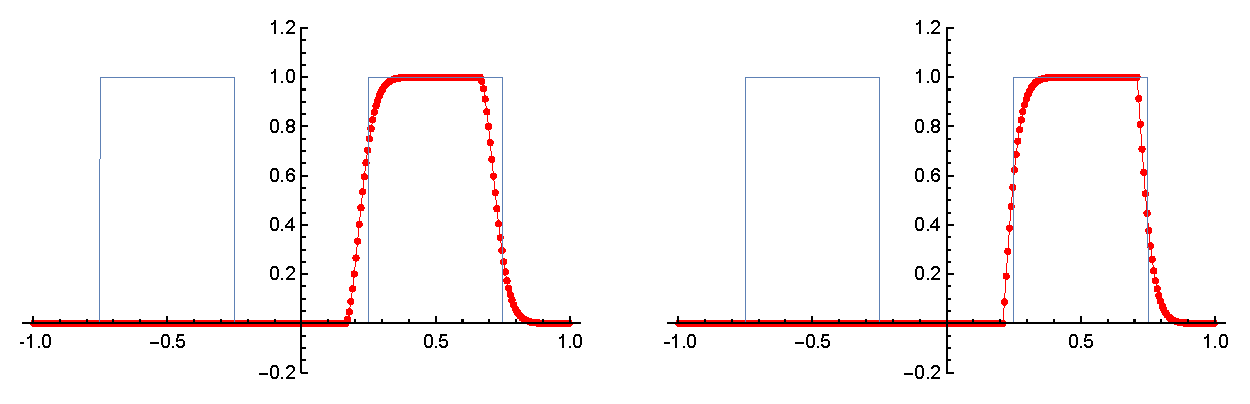
\includegraphics[width=\textwidth]{figures/compareDisc.pdf}
	\caption{Comparing the $\mathrm{S^1 IIOE}$ (without quadratic reconstruction) and the $\mathrm{FLIIOE}$ schemes with the exact solution  in time $ t=1 $, $ n=320 $, $ \tau=h $.}
	\label{fig:compare_S1FL_disc}
\end{figure}

\subsection{Inviscid Burgers' equation}
We performed numerical experiments also for the nonlinear transport equation \eqref{inviscid}. First we chose an exact solution that is smooth for $ t \geq 0 $ to show that the basic IIOE scheme is second order accurate in that case.  The other three examples are for testing the flux limited scheme. For this purpose the following examples where chosen: shock wave, rarefaction wave and triangular wave. \\

\textbf{Smooth rarefaction}. In order to have some experimental evidence that the IIOE scheme is second order accuraet for conservation laws of the form \eqref{scalar_conservation}, we chose a smooth rarefaction wave solution for the inviscid Burgers' equation \eqref{inviscid} with given initial condition
\[
u_0(x) = \frac{\arctan (10\,x) }{\pi} + 1/2.
\]
The exact solution can be obtained by the method of characteristics, see e.g.\ \cite{olv, lev, whitham}. It can be shown, that if the initial profile is non-decreasing $ u_0'(x) \geq 0 $ everywhere, then the solution doesn't develop discontinuities for $ t>0 $ \cite{olv, whitham}. The numerical solution was computed on space interval (-2, 2) and time (0, 1). The $ L_1(I, L_1) $ errors and EOC are reported in \ref{tab:fliioe_smooth}.
\begin{table}[ht]
	\caption{Report on the $L_1(I, L_1)$ errors of the $\mathrm{IIOE}$ scheme for a smooth rarefaction wave solution of the inviscid Burgers' equation, $ \tau = 4h $.}
	\begin{center} \footnotesize
		\begin{tabular}{|c|c|c|c|c|c|}
			\hline
			$ n $ & $ h $ & $ \tau $ & NTS& $\mathrm{L_1(I,L_1)}$ & EOC \\
			\hline
			\lower.3ex\hbox{80} & \lower.3ex\hbox{0.05} & \lower.3ex\hbox{0.2} & \lower.3ex\hbox{5} & \lower.3ex\hbox{2.32 $10^{-2}$} & \\
			\hline
			\lower.3ex\hbox{160} & \lower.3ex\hbox{0.025} & \lower.3ex\hbox{0.1} & \lower.3ex\hbox{10} & \lower.3ex\hbox{6.93 $10^{-3}$} &\lower.3ex\hbox{1.74} \\
			\hline
			\lower.3ex\hbox{320} & \lower.3ex\hbox{0.0125} & \lower.3ex\hbox{0.05} & \lower.3ex\hbox{20} & \lower.3ex\hbox{1.86 $10^{-3}$}  &\lower.3ex\hbox{1.90}\\
			\hline
			\lower.3ex\hbox{640} & \lower.3ex\hbox{0.00625} & \lower.3ex\hbox{0.025} & \lower.3ex\hbox{40} & \lower.3ex\hbox{4.70 $10^{-4}$}  &\lower.3ex\hbox{1.98}\\
			\hline
		\end{tabular}
	\end{center}
	\label{tab:fliioe_smooth}
\end{table}
\begin{figure}[H]
	\centering
	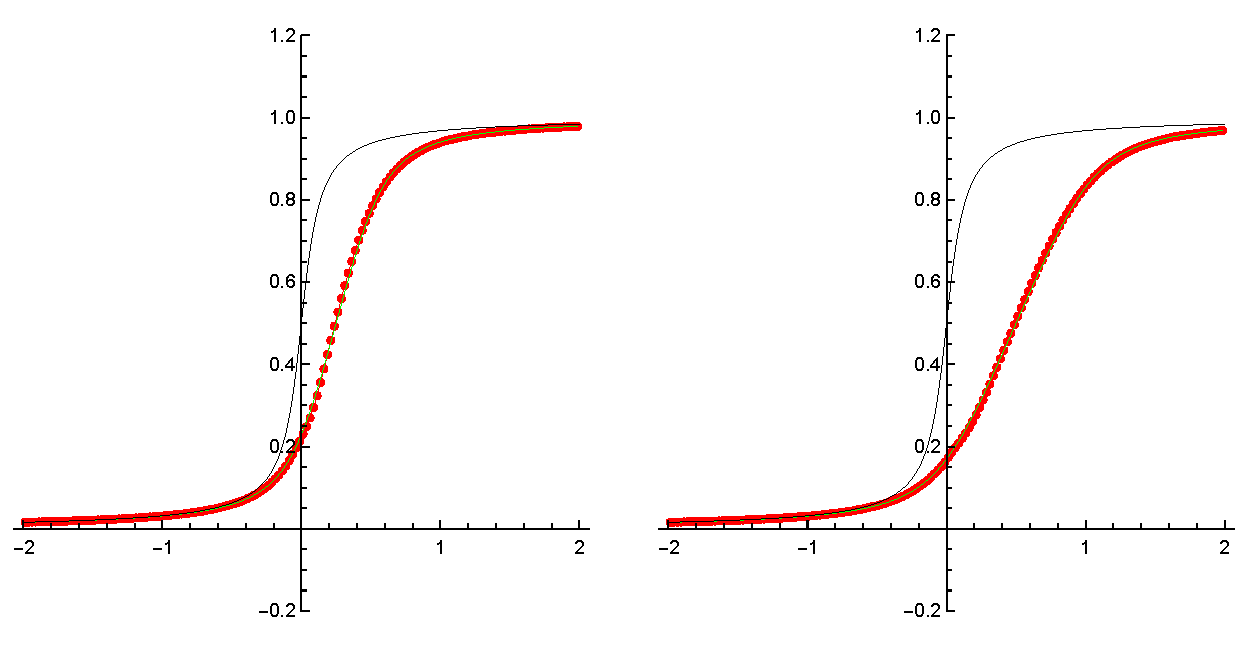
\includegraphics[width=\textwidth]{figures/invBurgSmooth160c4}
	\caption{Comparing the $\mathrm{IIOE}$ scheme with the exact smooth solution in time $ t=0.5 $(left) and $ t=1 $(right), $ n=160 $, $ \tau=4h $.}
	\label{fig:fliioe_burg_smooth}
\end{figure}

\textbf{Shock wave}. In this case the scheme \eqref{burgers_limit} is solved on the space interval $ (-0.5,\, 0.5) $ and time interval $ (0, 0.5) $ with a step function initial condition
\begin{equation}
	u_0(x) =
	\begin{cases}
		1, &x\leq 0,\nonumber\\
		0, &x>0.\nonumber
	\end{cases}
\end{equation}
A physically relevant weak solution\cite{olv, lev, whitham} is a traveling shock wave 
\[
u(t,x)=u_0(x - s\,t),
\]
where $ s = 1/2 $ is the speed of the shock propagation. The $ \mathrm{L_1(I,L_1)} $ errors and EOC of the computation are documented in \ref{tab:fliioe_invBurg_shock}. A visual comparison of the numerical solution with the exact one can be seen in \ref{fig:fliioe_burg_shock}.
\begin{table}[ht]
	\caption{Report on the $L_1(I,L_1)$ errors of the $\mathrm{FLIIOE}$(flux limited) scheme for a shock wave solution of the inviscid Burgers' equation. We used time steps $ \tau = 4h $ in the first 4 rows and $ \tau = 32h $ in the next 4 rows.}
	\begin{center} \footnotesize
		\begin{tabular}{|c|c|c|c|c|c|}
			\hline
			$ n $ & $ h $ & $ \tau $ & NTS& $\mathrm{L_1(I,L_1)}$ & EOC \\
			%c=4
			\hline
			\lower.3ex\hbox{80} & \lower.3ex\hbox{0.0125} & \lower.3ex\hbox{0.05} & \lower.3ex\hbox{10} & \lower.3ex\hbox{5.03 $10^{-3}$} & \\
			\hline
			\lower.3ex\hbox{160} & \lower.3ex\hbox{0.0125} & \lower.3ex\hbox{0.025} & \lower.3ex\hbox{20} & \lower.3ex\hbox{2.52 $10^{-3}$} &\lower.3ex\hbox{0.99} \\
			\hline
			\lower.3ex\hbox{320} & \lower.3ex\hbox{0.003125} & \lower.3ex\hbox{0.0125} & \lower.3ex\hbox{40} & \lower.3ex\hbox{1.26 $10^{-3}$}  &\lower.3ex\hbox{1.00}\\
			\hline
			\lower.3ex\hbox{640} & \lower.3ex\hbox{0.0015625} & \lower.3ex\hbox{0.00625} & \lower.3ex\hbox{80} & \lower.3ex\hbox{6.32 $10^{-3}$}  &\lower.3ex\hbox{1.00}\\
			\hline \hline
			%c=
			\lower.3ex\hbox{320} & \lower.3ex\hbox{0.03125} & \lower.3ex\hbox{0.1} & \lower.3ex\hbox{5} & \lower.3ex\hbox{6.78 $10^{-3}$} & \\
			\hline
			\lower.3ex\hbox{640} & \lower.3ex\hbox{0.0015625} & \lower.3ex\hbox{0.05} & \lower.3ex\hbox{10} & \lower.3ex\hbox{3.39 $10^{-3}$} &\lower.3ex\hbox{1.00} \\
			\hline
			\lower.3ex\hbox{1280} & \lower.3ex\hbox{0.00078125} & \lower.3ex\hbox{0.025} & \lower.3ex\hbox{20} & \lower.3ex\hbox{1.69 $10^{-3}$}  &\lower.3ex\hbox{1.00}\\
			\hline
			\lower.3ex\hbox{2560} & \lower.3ex\hbox{0.000391} & \lower.3ex\hbox{0.0125} & \lower.3ex\hbox{40} & \lower.3ex\hbox{8.47 $10^{-4}$}  &\lower.3ex\hbox{1.00}\\
			\hline
		\end{tabular}
	\end{center}
	\label{tab:fliioe_invBurg_shock}
\end{table}
\begin{figure}[H]
	\centering
	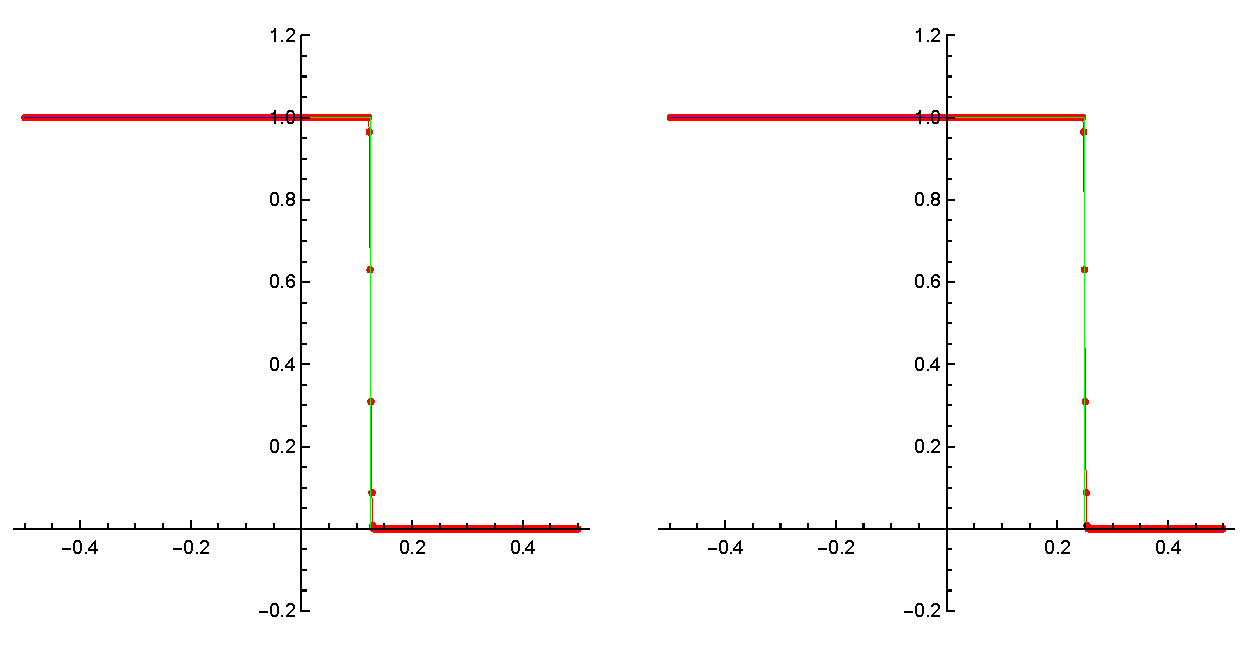
\includegraphics[width=.9\textwidth]{figures/inviscidShock640c4}
	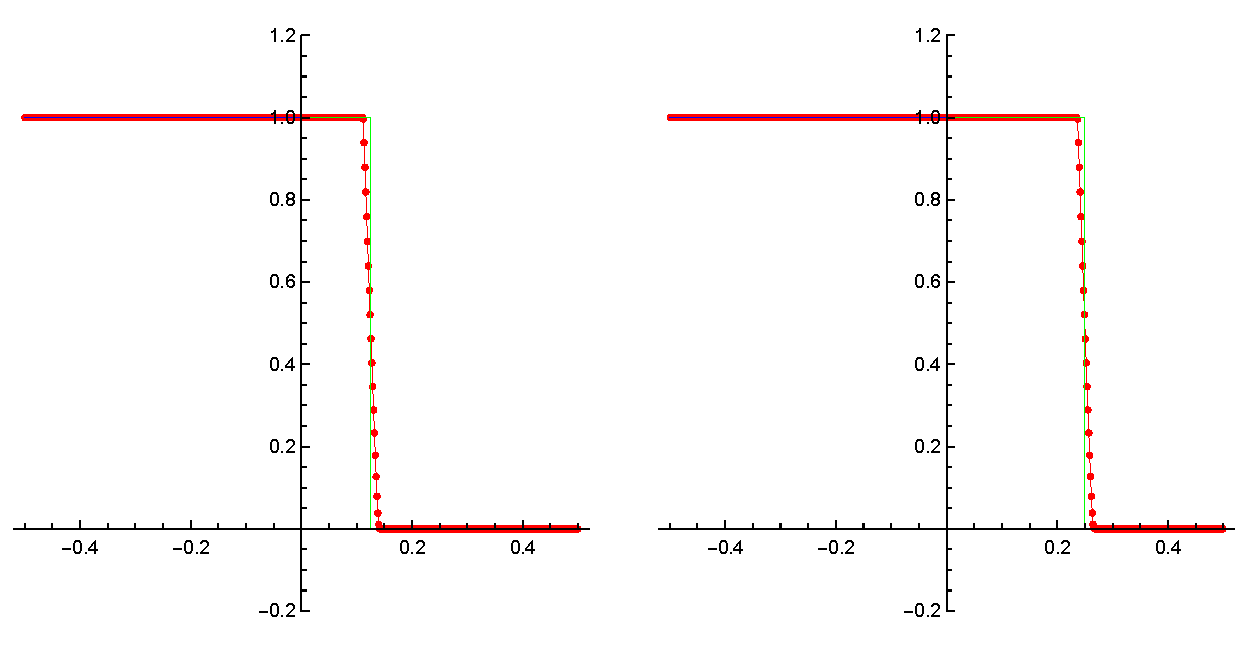
\includegraphics[width=.9\textwidth]{figures/inviscidShock640c32}
	\caption{Results of the $\mathrm{FLIIOE}$(flux limited) scheme with the traveling shock wave solution at time $ t=0.25 $(left) and $ t=0.5 $(right), $ n=640 $ for relatively large time steps $ \tau=4h $(top), $ \tau=32h $(bottom). The initial profile is given in black, the exact solution in green and the numerical solution in red.}
	\label{fig:fliioe_burg_shock}
\end{figure}

\textbf{Rarefaction wave}. The next example is a solution of \eqref{inviscid} with a discontinous initial condition
\begin{equation}
	u_0(x) =
	\begin{cases}
		0, &x\leq 0,\nonumber\\
		1, &x>0.\nonumber
	\end{cases}
\end{equation}
A physically relevant solution is a rarefaction wave\cite{olv, lev, whitham} for $ t>0 $
\begin{equation}
	u(t,x) =
	\begin{cases}
		1, &x>t,\nonumber\\
		x/t, &0 \leq x \leq t,\nonumber\\
		0, &x<0.\nonumber
	\end{cases}
\end{equation}
We solved \eqref{inviscid} numerically by \eqref{burgers_limit} on space interval (-0.5, 1.5) and time interval (0, 1). The results are documented in \ref{tab:fliioe_rare}. The numerical solution is compared visually with the exact one in \ref{fig:fliioe_shock_rare}.
\begin{table}[ht]
	\caption{Report on the $L_1(I,L_1)$ errors of the $\mathrm{FLIIOE}$(flux limited) scheme for a rarefaction wave solution of the inviscid Burgers' equation. We used time steps $ \tau=h $(top), $ \tau=2h $(bottom).}
	\begin{center} \footnotesize
		\begin{tabular}{|c|c|c|c|c|c|}
			\hline
			$ n $ & $ h $ & $ \tau $ & NTS& $\mathrm{L_1(I,L_1)}$ & EOC \\
			\hline
			\lower.3ex\hbox{80} & \lower.3ex\hbox{0.025} & \lower.3ex\hbox{0.025} & \lower.3ex\hbox{40} & \lower.3ex\hbox{1.63 $10^{-2}$} & \\
			\hline
			\lower.3ex\hbox{160} & \lower.3ex\hbox{0.0125} & \lower.3ex\hbox{0.0125} & \lower.3ex\hbox{80} & \lower.3ex\hbox{8.90 $10^{-3}$} &\lower.3ex\hbox{0.87} \\
			\hline
			\lower.3ex\hbox{320} & \lower.3ex\hbox{0.00625} & \lower.3ex\hbox{0.00625} & \lower.3ex\hbox{160} & \lower.3ex\hbox{4.70 $10^{-3}$}  &\lower.3ex\hbox{0.92}\\
			\hline
			\lower.3ex\hbox{640} & \lower.3ex\hbox{0.003125} & \lower.3ex\hbox{0.003125} & \lower.3ex\hbox{320} & \lower.3ex\hbox{2.42 $10^{-3}$}  &\lower.3ex\hbox{0.96}\\
			\hline \hline
			\lower.3ex\hbox{80} & \lower.3ex\hbox{0.025} & \lower.3ex\hbox{0.05} & \lower.3ex\hbox{20} & \lower.3ex\hbox{2.21 $10^{-2}$} & \\
			\hline
			\lower.3ex\hbox{160} & \lower.3ex\hbox{0.0125} & \lower.3ex\hbox{0.025} & \lower.3ex\hbox{40} & \lower.3ex\hbox{1.22 $10^{-2}$} &\lower.3ex\hbox{0.86} \\
			\hline
			\lower.3ex\hbox{320} & \lower.3ex\hbox{0.00625} & \lower.3ex\hbox{0.0125} & \lower.3ex\hbox{80} & \lower.3ex\hbox{6.58 $10^{-3}$}  &\lower.3ex\hbox{0.89}\\
			\hline
			\lower.3ex\hbox{640} & \lower.3ex\hbox{0.00625} & \lower.3ex\hbox{0.003125} & \lower.3ex\hbox{160} & \lower.3ex\hbox{3.45 $10^{-3}$}  &\lower.3ex\hbox{0.93}\\
			\hline
		\end{tabular}
	\end{center}
	\label{tab:fliioe_rare}
\end{table}
\begin{figure}[H]
	\centering
	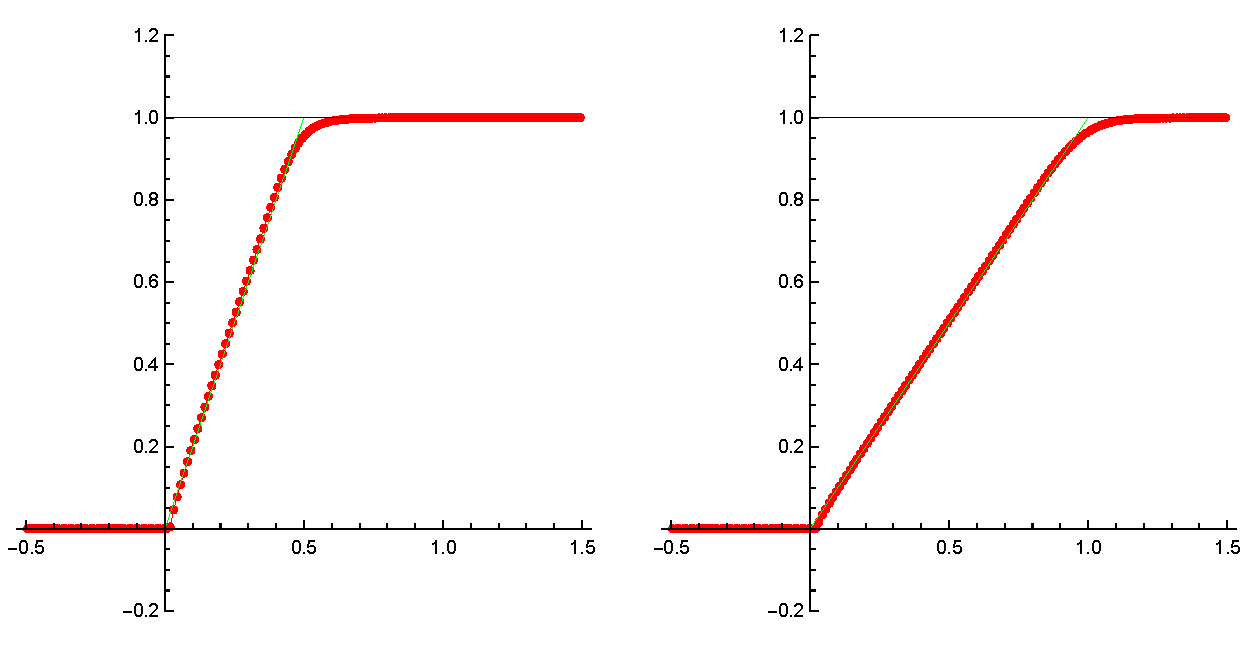
\includegraphics[width=\textwidth]{figures/inviscidRare160c1.pdf}
	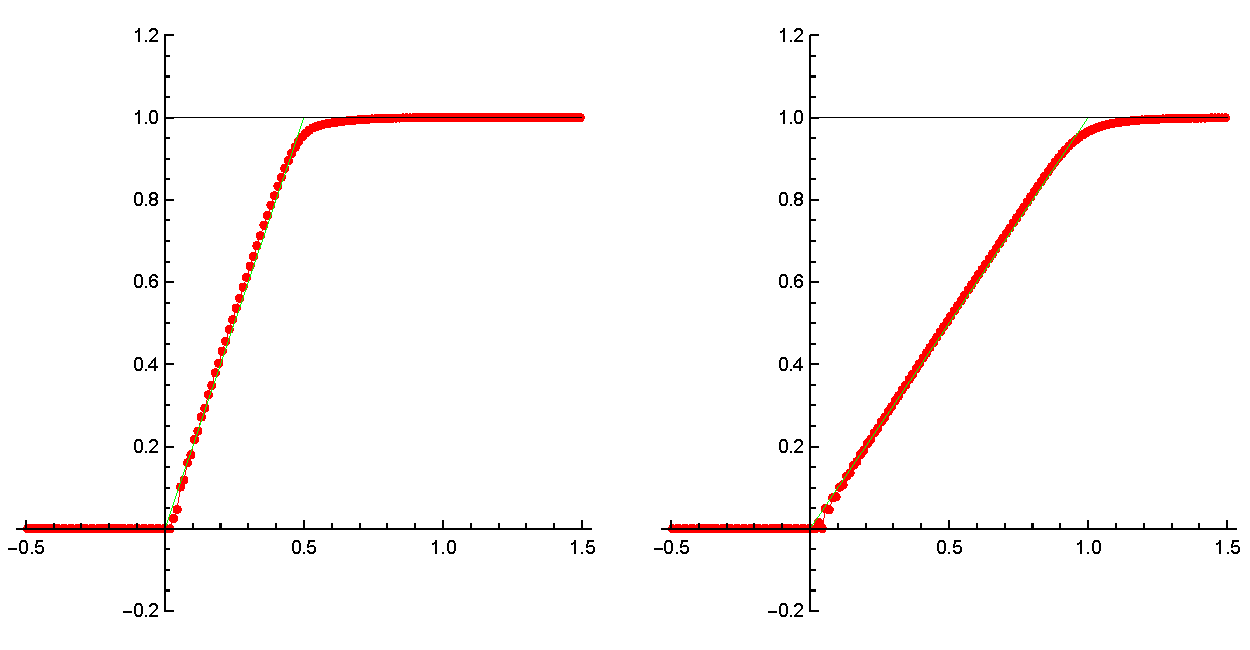
\includegraphics[width=\textwidth]{figures/inviscidRare160c2.pdf}
	\caption{Results of the $\mathrm{FLIIOE}$(flux limited) scheme for a rarefaction wave solution of the inviscid Burgers' equation at time $ t=0.5 $(left) and $ t=1 $(right), $ n=160 $. We used time steps $ \tau=h $(top), $ \tau=2h $(bottom). The initial profile is given in black, the exact solution in green and the numerical solution in red.}
	\label{fig:fliioe_shock_rare}
\end{figure}
\newpage
\textbf{Triangular wave}
The third example is a weak solution of \eqref{inviscid} \cite{olv, lev, whitham} given for $ t\geq0 $ as
\begin{equation}
	u(t,x) =
	\begin{cases}
		x/(1+t), &0 \leq x \leq \sqrt{1+t},\nonumber\\
		0, &otherwise.\nonumber
	\end{cases}
\end{equation}
We solved \eqref{inviscid} numerically by \eqref{burgers_limit} on space interval (-0.5, 1.5) and time interval (0, 1). The results are documented in \ref{tab:fliioe_triang}. The numerical solution is compared visually with the exact one in \ref{fig:fliioe_burg_triang}.
\begin{table}[ht]
	\caption{Report on the $L_1(I, L_1)$ errors of the $\mathrm{FLIIOE}$(flux limited) scheme for a triangular wave solution of the inviscid Burgers' equation, with time steps $ \tau = h $ in the first 4 rows and $ \tau = 2h $ in the next 4 rows.}
	\begin{center} \footnotesize
		\begin{tabular}{|c|c|c|c|c|c|}
			\hline
			$ n $ & $ h $ & $ \tau $ & NTS& $\mathrm{L_1(I,L_1)}$ & EOC \\
			\hline
			\lower.3ex\hbox{80} & \lower.3ex\hbox{0.025} & \lower.3ex\hbox{0.025} & \lower.3ex\hbox{40} & \lower.3ex\hbox{1.62 $10^{-2}$} & \\
			\hline
			\lower.3ex\hbox{160} & \lower.3ex\hbox{0.0125} & \lower.3ex\hbox{0.0125} & \lower.3ex\hbox{80} & \lower.3ex\hbox{7.73 $10^{-3}$} &\lower.3ex\hbox{1.07} \\
			\hline
			\lower.3ex\hbox{320} & \lower.3ex\hbox{0.00625} & \lower.3ex\hbox{0.00625} & \lower.3ex\hbox{160} & \lower.3ex\hbox{3.66 $10^{-3}$}  &\lower.3ex\hbox{1.08}\\
			\hline
			\lower.3ex\hbox{640} & \lower.3ex\hbox{0.003125} & \lower.3ex\hbox{0.003125} & \lower.3ex\hbox{320} & \lower.3ex\hbox{1.77 $10^{-3}$}  &\lower.3ex\hbox{1.05}\\
			\hline \hline
			\lower.3ex\hbox{80} & \lower.3ex\hbox{0.025} & \lower.3ex\hbox{0.05} & \lower.3ex\hbox{20} & \lower.3ex\hbox{2.40 $10^{-2}$} & \\
			\hline
			\lower.3ex\hbox{160} & \lower.3ex\hbox{0.0125} & \lower.3ex\hbox{0.025} & \lower.3ex\hbox{40} & \lower.3ex\hbox{1.14 $10^{-2}$} &\lower.3ex\hbox{1.07} \\
			\hline
			\lower.3ex\hbox{320} & \lower.3ex\hbox{0.00625} & \lower.3ex\hbox{0.0125} & \lower.3ex\hbox{80} & \lower.3ex\hbox{5.35 $10^{-3}$}  &\lower.3ex\hbox{1.09}\\
			\hline
			\lower.3ex\hbox{640} & \lower.3ex\hbox{0.00625} & \lower.3ex\hbox{0.003125} & \lower.3ex\hbox{160} & \lower.3ex\hbox{2.66 $10^{-3}$}  &\lower.3ex\hbox{1.01}\\
			\hline
		\end{tabular}
	\end{center}
	\label{tab:fliioe_triang}
\end{table}
\begin{figure}[H]
	\centering
	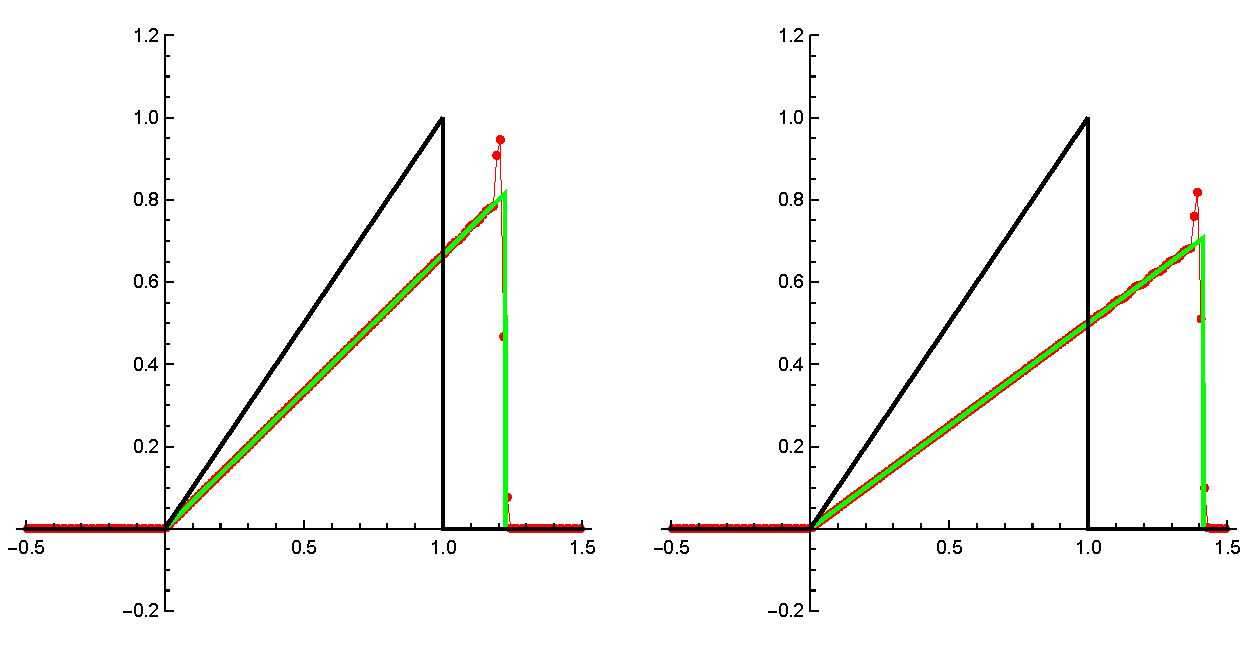
\includegraphics[width=\textwidth]{figures/inviscidTriang160c1}
	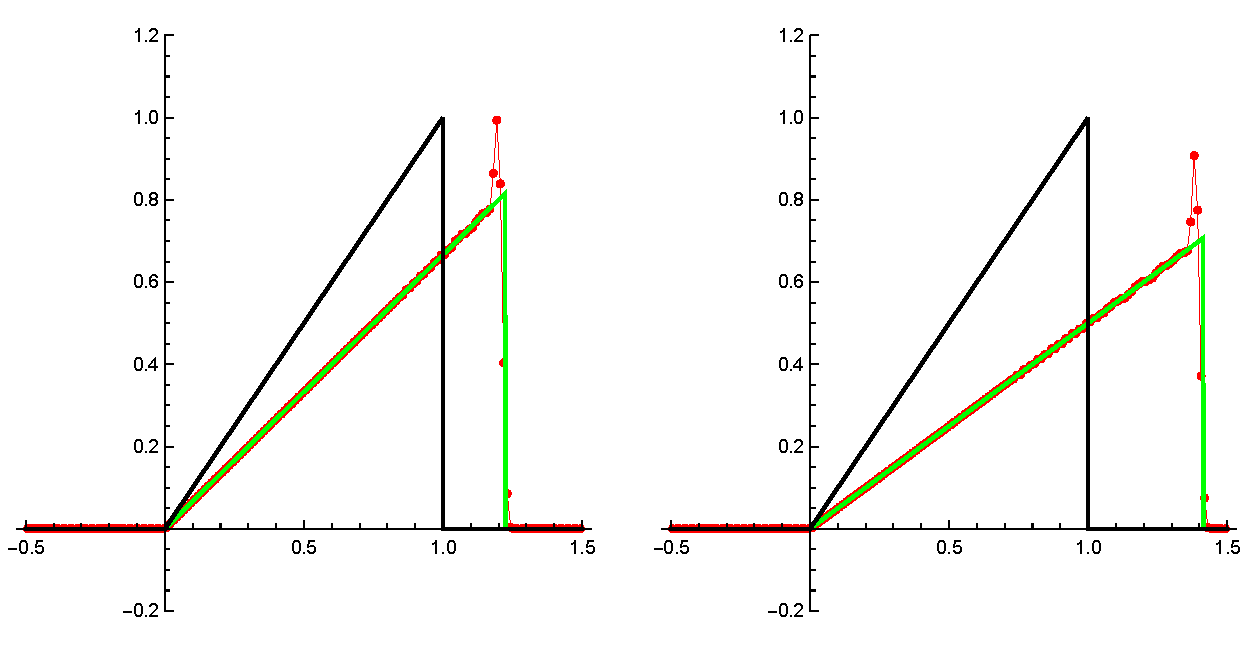
\includegraphics[width=\textwidth]{figures/inviscidTriang160c2}
	\caption{Results of the $\mathrm{FLIIOE}$(flux limited) scheme for a triangular wave solution of the inviscid Burgers' equation at time $ t=0.5 $(left) and $ t=1 $(right), $ n=160 $. We used time steps $ \tau=h $(top), $ \tau=2h $(bottom). The initial profile is given in black, the exact solution in green and the numerical solution in red..}
	\label{fig:fliioe_burg_triang}
\end{figure}
%====================================================================================================================================================
\chapter{Thesis objectives and prospective contribution}
\chaptermark{Thesis objectives}
In the future we plan to perform the following tasks:
\begin{itemize}
	\item Improving the flux-limiting process, extension to 2D, 3D
	\item Comparing the performance with other schemes
	\item Test the scheme on higher order models of traffic flow
	\item Using the scheme for computing traffic flow on networks
\end{itemize}
%====================================================================================================================================================
\end{document}